\documentclass[12pt,letterpaper]{article}
\usepackage{graphicx,textcomp}
\usepackage{natbib}
\usepackage{setspace}
\usepackage{fullpage}
\usepackage{color}
\usepackage[reqno]{amsmath}
\usepackage{amsthm}
\usepackage{fancyvrb}
\usepackage{amssymb,enumerate}
\usepackage[all]{xy}
\usepackage{endnotes}
\usepackage{lscape}
\newtheorem{com}{Comment}
\usepackage{float}
\usepackage{hyperref}
\newtheorem{lem} {Lemma}
\newtheorem{prop}{Proposition}
\newtheorem{thm}{Theorem}
\newtheorem{defn}{Definition}
\newtheorem{cor}{Corollary}
\newtheorem{obs}{Observation}
\usepackage[compact]{titlesec}
\usepackage{dcolumn}
\usepackage{tikz}
\usetikzlibrary{arrows}
\usepackage{multirow}
\usepackage{xcolor}
\newcolumntype{.}{D{.}{.}{-1}}
\newcolumntype{d}[1]{D{.}{.}{#1}}
\definecolor{light-gray}{gray}{0.65}
\usepackage{url}
\usepackage{listings}
\usepackage{color}

\definecolor{codegreen}{rgb}{0,0.6,0}
\definecolor{codegray}{rgb}{0.5,0.5,0.5}
\definecolor{codepurple}{rgb}{0.58,0,0.82}
\definecolor{backcolour}{rgb}{0.95,0.95,0.92}

\lstdefinestyle{mystyle}{
	backgroundcolor=\color{backcolour},   
	commentstyle=\color{codegreen},
	keywordstyle=\color{magenta},
	numberstyle=\tiny\color{codegray},
	stringstyle=\color{codepurple},
	basicstyle=\footnotesize,
	breakatwhitespace=false,         
	breaklines=true,                 
	captionpos=b,                    
	keepspaces=true,                 
	numbers=left,                    
	numbersep=5pt,                  
	showspaces=false,                
	showstringspaces=false,
	showtabs=false,                  
	tabsize=2
}
\lstset{style=mystyle}
\newcommand{\Sref}[1]{Section~\ref{#1}}
\newtheorem{hyp}{Hypothesis}

\title{\textbf{Problem Set 3}}
\date{\textbf{Due: November 12, 2026}}
\author{\textbf{Applied Stats/Quant Methods 1}}


\begin{document}
	\maketitle
	\section*{Instructions}
	\begin{itemize}
		\item Please show your work! You may lose points by simply writing in the answer. If the problem requires you to execute commands in \texttt{R}, please include the code you used to get your answers. Please also include the \texttt{.R} file that contains your code. If you are not sure if work needs to be shown for a particular problem, please ask.
	\item Your homework should be submitted electronically on GitHub.
	\item This problem set is due before 23:59 on Thursday November 12, 2026. No late assignments will be accepted.

	\end{itemize}

		\vspace{.25cm}
	
\noindent In this problem set, you will run several regressions and create an add variable plot (see the lecture slides) in \texttt{R} using the \texttt{incumbents\_subset.csv} dataset. Include all of your code.

	\vspace{.5cm}
\section*{Question 1}
\vspace{.25cm}
\noindent \textbf{We are interested in knowing how the difference in campaign spending between incumbent and challenger affects the incumbent's vote share.}
	\begin{enumerate}
		\item \textbf{Run a regression where the outcome variable is \texttt{voteshare} and the explanatory variable is \texttt{difflog}.}	\vspace{0cm}
		
		I used the built-in R function \texttt{lm()} to run the regression for Question $1$, using \texttt{voteshare} as the outcome (Y) variable and \texttt{difflog} as the explanatory (X) variable, where \texttt{voteshare} is the incumbent's proportion of the vote and \texttt{difflog} is the log difference in campaign spending between the incumbent and the challenger. 
		
		\lstinputlisting[language=R, firstline=51, lastline=52]{PS03_Solutions_AV.R} 
		
		I estimated that the y-intercept is $0.57903$ and $\hat{\beta}$ is $0.04167$. This means that when \texttt{difflog} is equal to 0, the predicted \texttt{voteshare} value is $0.58$ (rounded to $2$ d.p.). Furthermore, for every one unit increase in the \texttt{difflog}, there is a $0.04$ (rounded to $2$ d.p.) expected increase in \texttt{voteshare}.
		
		\item \textbf{Make a scatterplot of the two variables and add the regression line.} 	\vspace{0cm}
		
		I used \texttt{ggplot()} to make a scatterplot of these two variables. The graph in Figure 1 shows the linear relationship between \texttt{difflog} and \texttt{voteshare}. There is a clear positive relationship, meaning that as the log difference in campaign spending between the incumbent and the challenger increases, the incumbent's proportion of the vote increases, too. There is moderate scatter, with the majority of data clustered between \texttt{difflog} values of $-1$ and log $4$.
		
		\lstinputlisting[language=R, firstline=57, lastline=65]{PS03_Solutions_AV.R}  
		
		\begin{figure}[H]
			\centering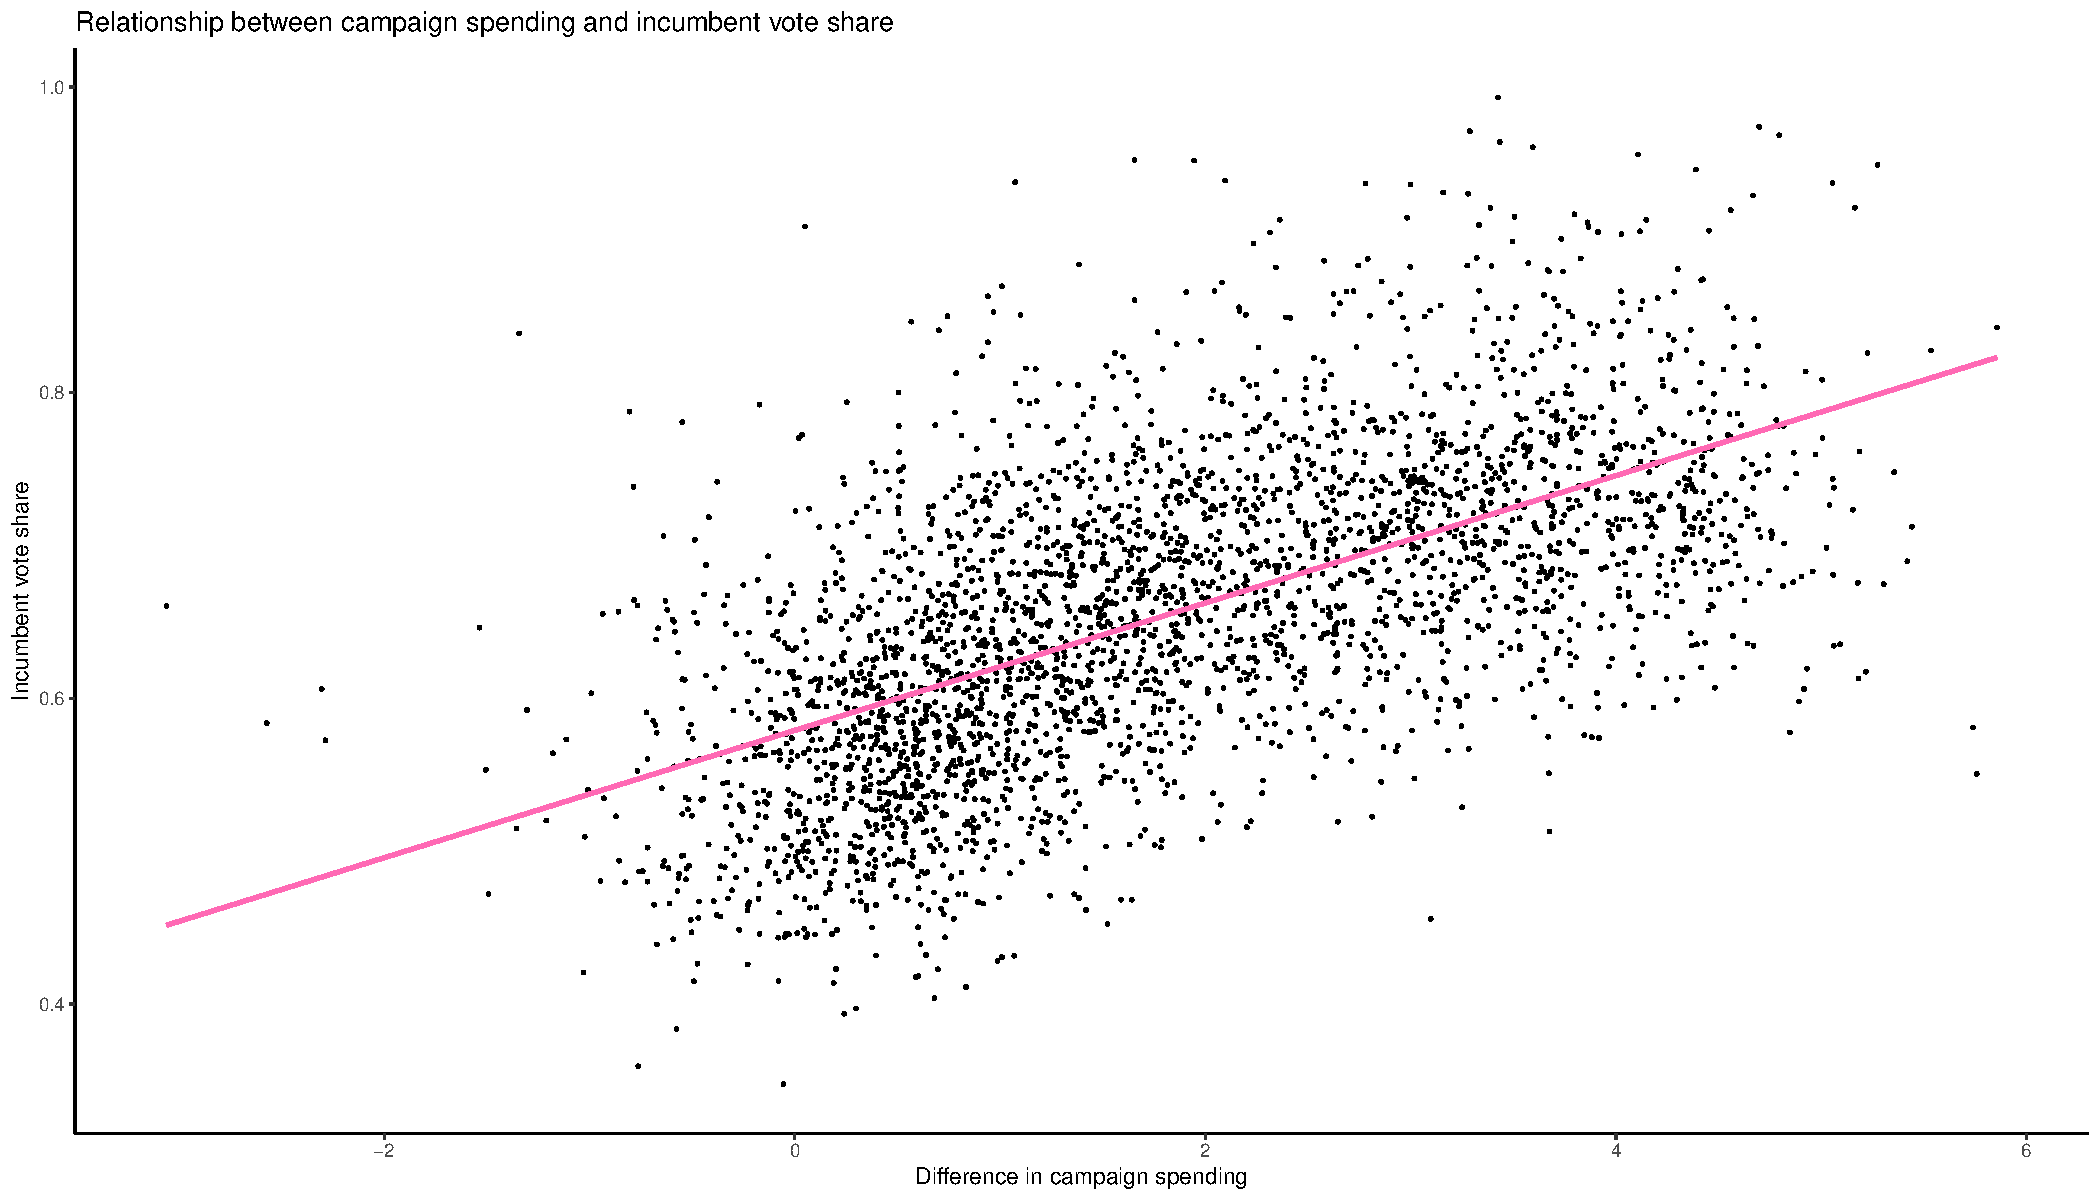
\includegraphics[width=0.95\linewidth]{P3_graph_1.pdf}
			\caption{Relationship between campaign spending and incumbent vote share}
		\end{figure}
		
		\item \textbf{Save the residuals of the model in a separate object.}	\vspace{0cm}
		
		Residuals are the difference between the observed \texttt{voteshare} and the \texttt{voteshare} predicted by the regression model. I used the built-in R function \texttt{residuals()} to calculate the residuals from the regression values I estimated in the first part of Question $1$. I stored the residuals in a new vector called \texttt{residuals\_1}.
		
		\lstinputlisting[language=R, firstline=70, lastline=71]{PS03_Solutions_AV.R}  
		
		\item \textbf{Write the prediction equation.}
		
		Using the values of y-intercept and $\hat{\beta}$ estimated from the regression model above, the prediction equation is:
		
		$$\widehat{\text{voteshare}} = 0.58 + 0.04 \cdot \text{difflog}$$
		
	\end{enumerate}
	
\newpage

\section*{Question 2}
\noindent \textbf{We are interested in knowing how the difference between incumbent and challenger's spending and the vote share of the presidential candidate of the incumbent's party are related.}	\vspace{.25cm}
	\begin{enumerate}
		\item \textbf{Run a regression where the outcome variable is \texttt{presvote} and the explanatory variable is \texttt{difflog}.}	\vspace{0cm}
		
		I used the built-in R function \texttt{lm()} to run the regression for Question $2$, using \texttt{presvote} as the outcome (Y) variable and \texttt{difflog} as the explanatory (X) variable, where \texttt{presvote} is the voteshare of the presidential candidate from the incumbent party and \texttt{difflog} is the log difference in campaign spending between the incumbent and the challenger. 
		
		\lstinputlisting[language=R, firstline=86, lastline=87]{PS03_Solutions_AV.R}  
		
		I estimated that the y-intercept is $0.50758$ and $\hat{\beta}$ is $0.02384$. This means that when \texttt{difflog} is equal to 0, the predicted \texttt{presvote} value is $0.51$ (rounded to $2$ d.p.). Furthermore, for every one unit increase in the \texttt{difflog}, there is a $0.02$ (rounded to $2$ d.p.) expected increase in \texttt{presvote}.
		
		\item \textbf{Make a scatterplot of the two variables and add the regression line.} 	\vspace{0cm}
		
		I used \texttt{ggplot()} to make a scatterplot of these two variables. The graph in Figure 1 shows the relationship between \texttt{difflog} and \texttt{presvote}. There is a positive linear relationship, meaning that as the log difference in campaign spending between the incumbent and the challenger increases, the voteshare of the presidential candidate from the incumbent party increases, too. The regression line is flatter in Figure 2 than in Figure 1, suggesting a weaker correlation between these variables. The data is also more scattered than in Figure 1.
		
		\lstinputlisting[language=R, firstline=92, lastline=100]{PS03_Solutions_AV.R}  
		
		\begin{figure}[H]
			\centering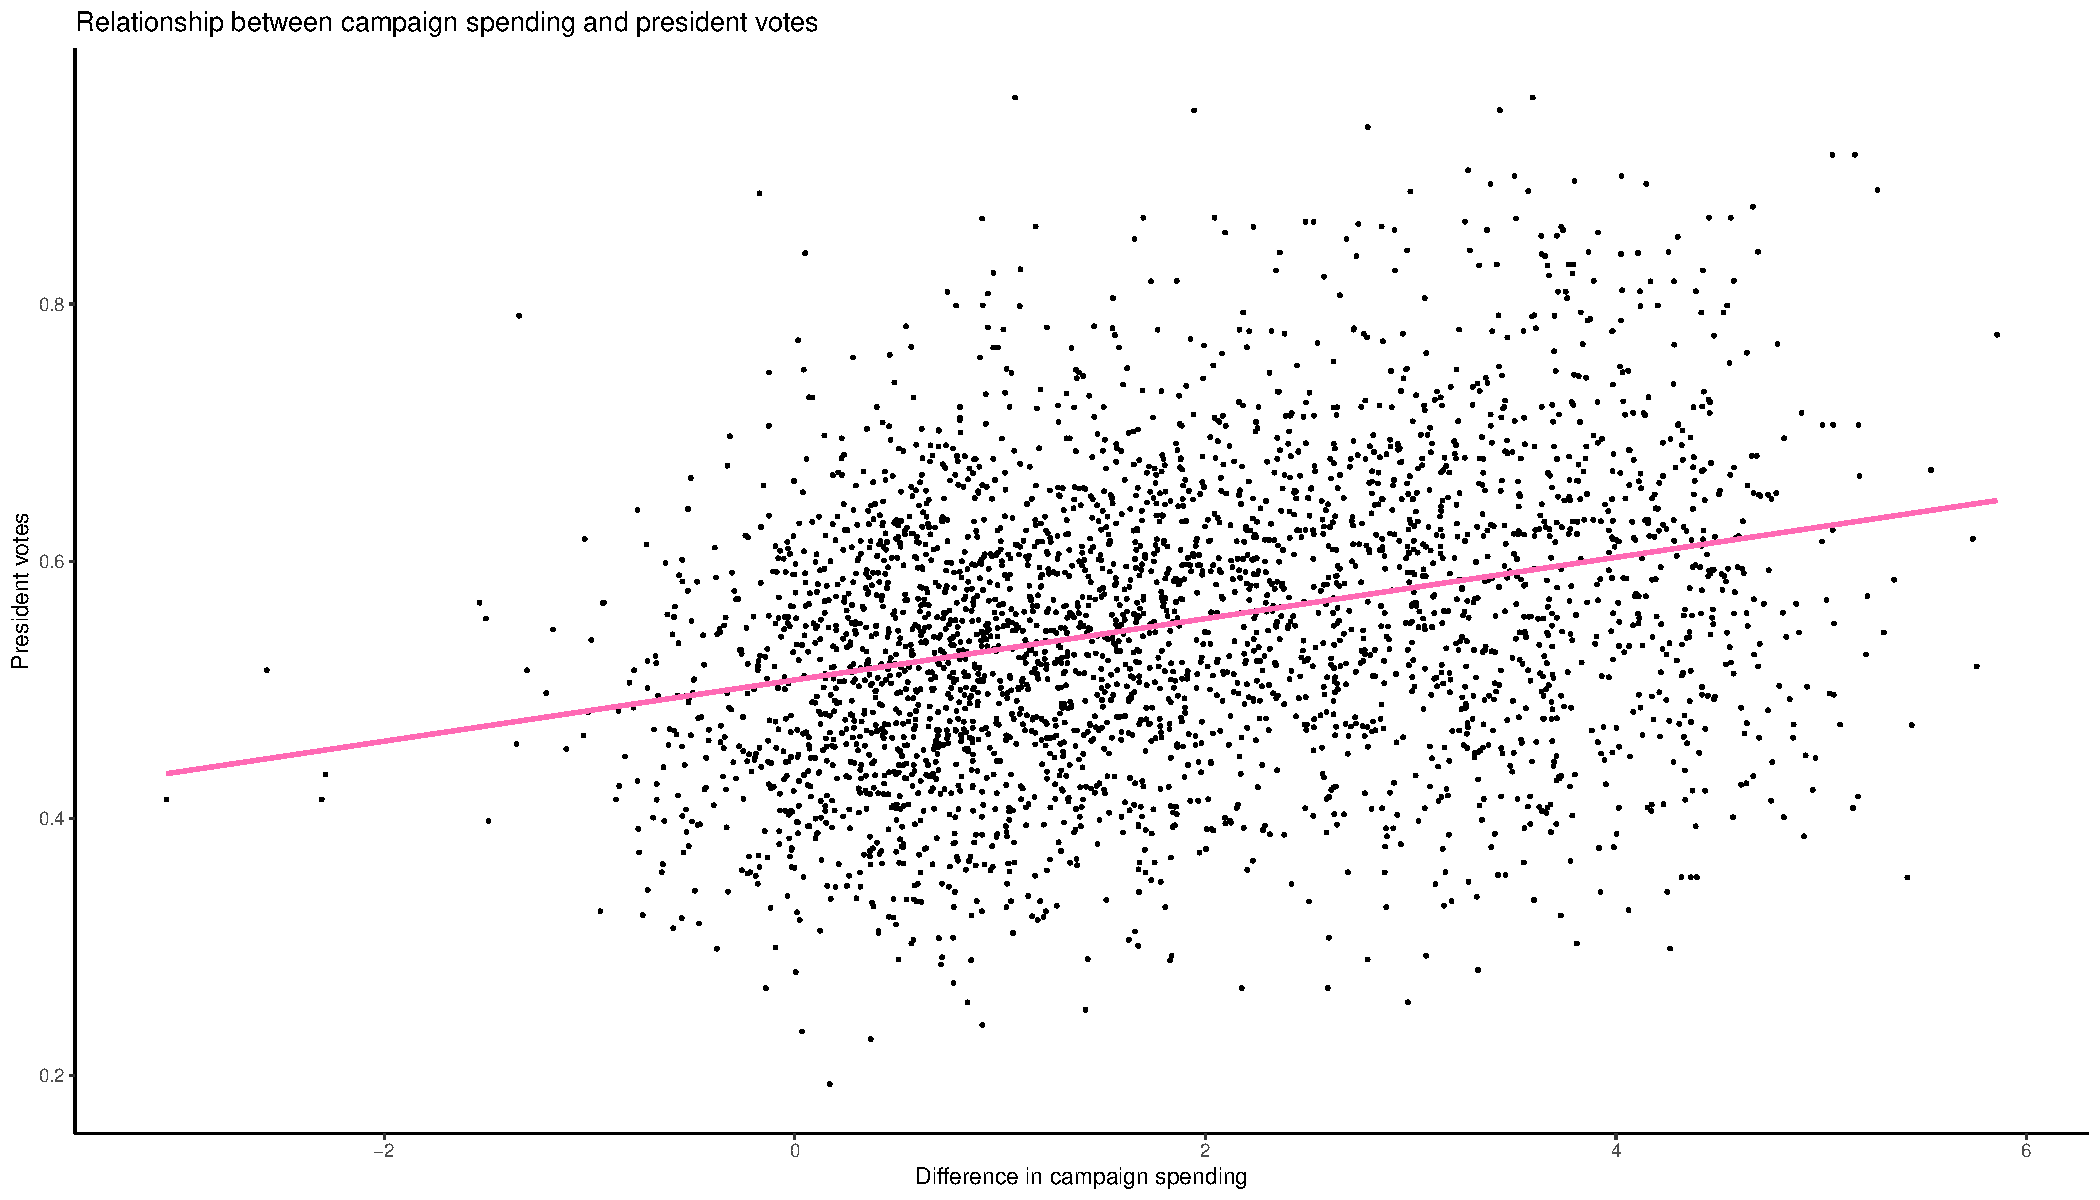
\includegraphics[width=0.95\linewidth]{P3_graph_2.pdf}
			\caption{Relationship between campaign spending and president votes}
		\end{figure}
		
		\item \textbf{Save the residuals of the model in a separate object.}	\vspace{0cm}
		
		Residuals are the difference between the observed \texttt{presvote} and the \texttt{presvote} predicted by the regression model. As in Question 1, I used the built-in R function \texttt{residuals()} and stored the residuals in a new vector called \texttt{residuals\_2}.
		
		\lstinputlisting[language=R, firstline=105, lastline=106]{PS03_Solutions_AV.R}  
		
		\item \textbf{Write the prediction equation.}
		
		Using the values of y-intercept and $\hat{\beta}$ estimated from the regression model above, the prediction equation is:
		
		$$\widehat{\text{presvote}} = 0.51 + 0.02 \cdot \text{difflog}$$
		
	\end{enumerate}
	
	\newpage	
\section*{Question 3}

\noindent \textbf{We are interested in knowing how the vote share of the presidential candidate of the incumbent's party is associated with the incumbent's electoral success.}
	\vspace{.25cm}
	\begin{enumerate}
		\item \textbf{Run a regression where the outcome variable is \texttt{voteshare} and the explanatory variable is \texttt{presvote}.}
			\vspace{0cm}
			
			I used the built-in R function \texttt{lm()} to run the regression for Question $3$, using \texttt{voteshare} as the outcome (Y) variable and \texttt{presvote} as the explanatory (X) variable, where \texttt{voteshare} is the incumbent's proportion of the vote and \texttt{presvote} is the voteshare of the presidential candidate from the incumbent party.
			
			\lstinputlisting[language=R, firstline=122, lastline=123]{PS03_Solutions_AV.R}  
			
			I estimated that the y-intercept is $0.4413$ and $\hat{\beta}$ is $0.3880$. This means that when \texttt{presvote} is equal to 0, the predicted \texttt{voteshare} value is $0.44$ (rounded to $2$ d.p.). Furthermore, for every one unit increase in the \texttt{presvote}, there is a $0.39$ (rounded to $2$ d.p.) expected increase in \texttt{voteshare}.
			
		\item \textbf{Make a scatterplot of the two variables and add the regression line.} 
			\vspace{0cm}
			
			I used \texttt{ggplot()} to make a scatterplot of these two variables. The graph in Figure $3$ shows the relationship between \texttt{presvote} and \texttt{voteshare}. There is a strong positive linear relationship, meaning that as the voteshare of the presidential candidate from the incumbent party increases, so too does the incumbent's proportion of the vote.
			
			\lstinputlisting[language=R, firstline=128, lastline=136]{PS03_Solutions_AV.R}  
			
			\begin{figure}[H]
				\centering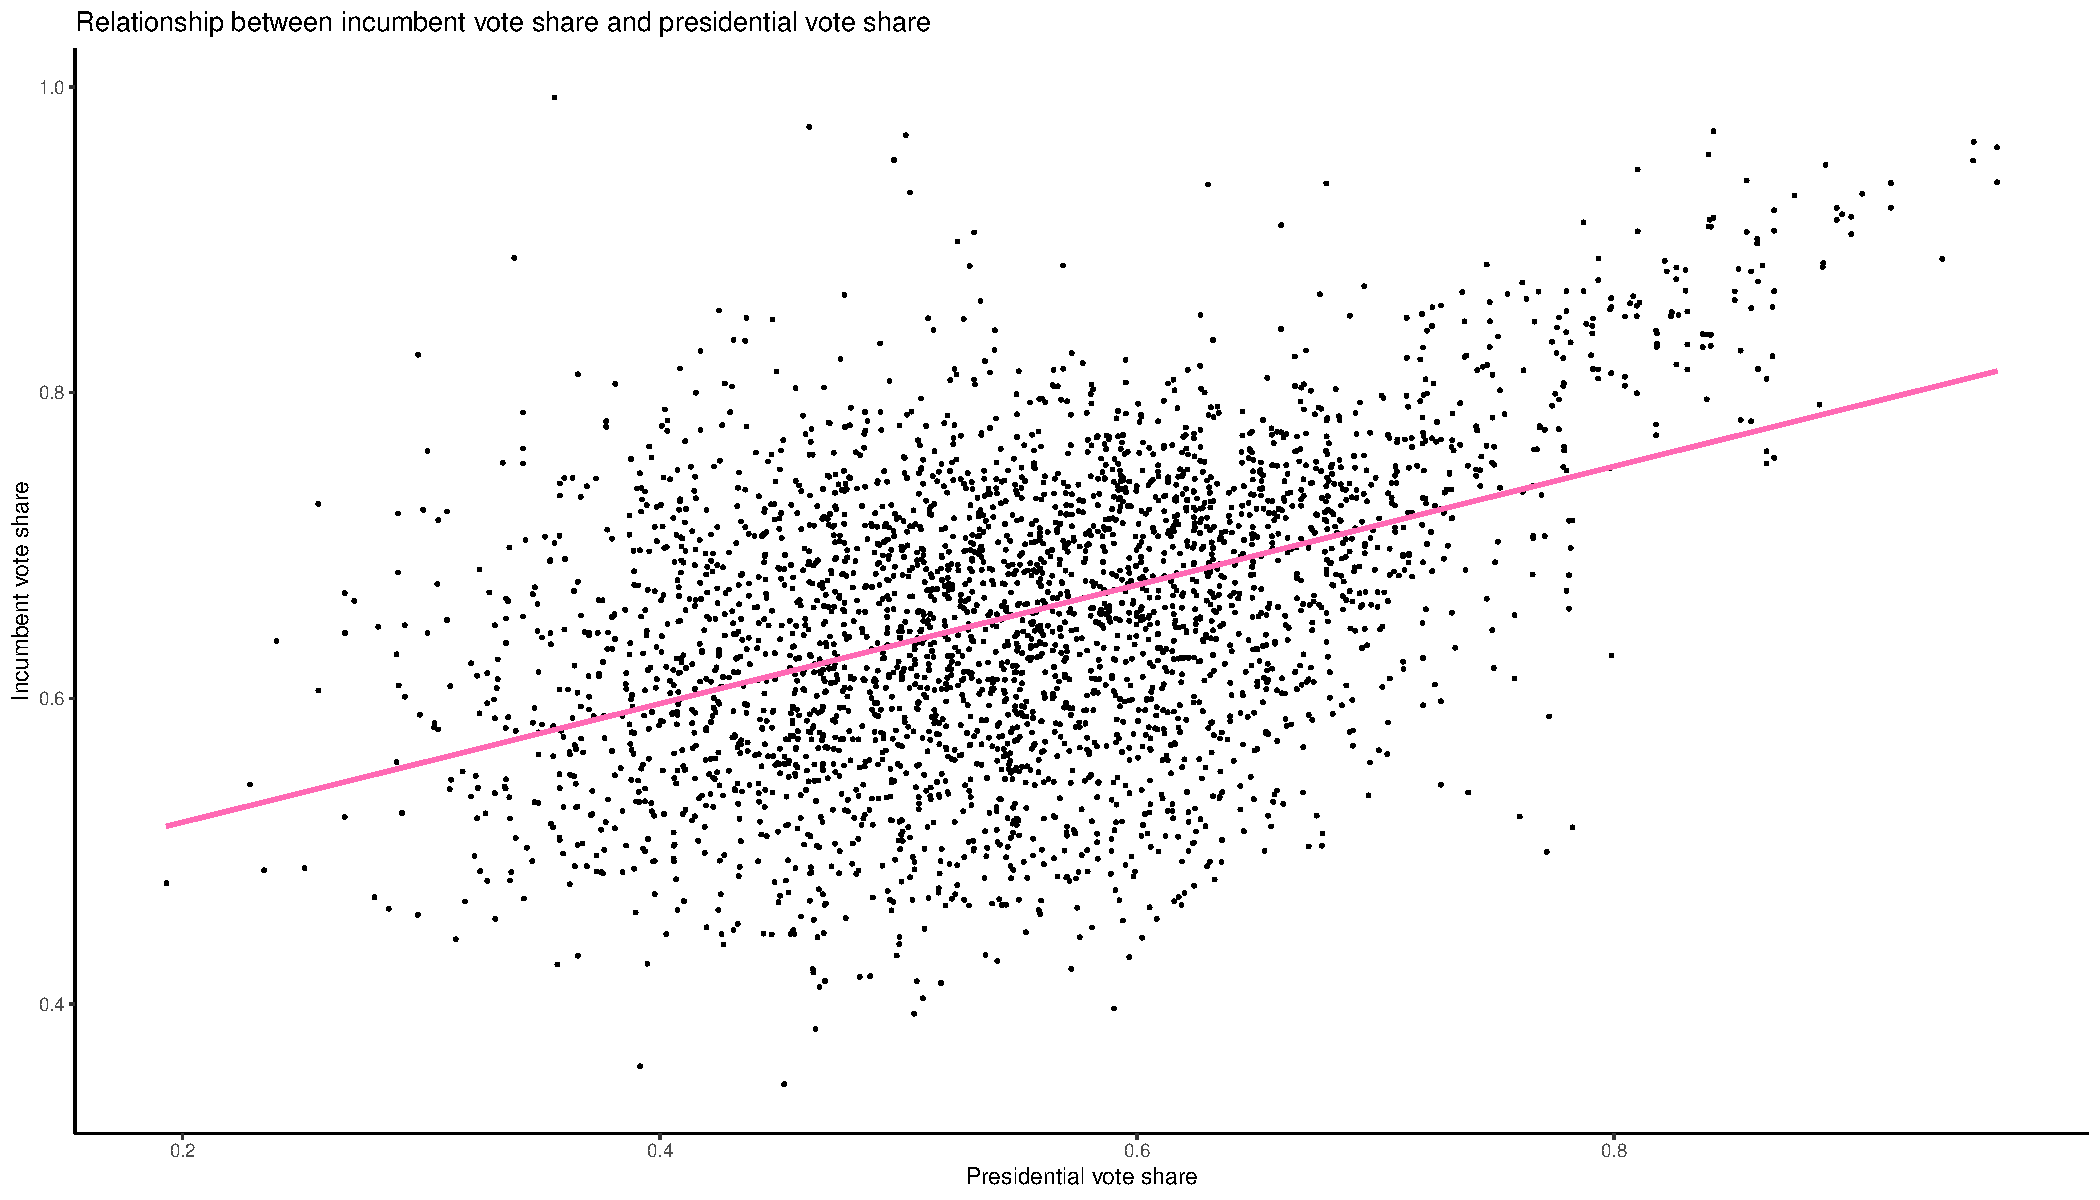
\includegraphics[width=0.95\linewidth]{P3_graph_3.pdf}
				\caption{Relationship between incumbent vote share and president votes}
			\end{figure}
			
		\item \textbf{Write the prediction equation.}
		
		Using the values of y-intercept and $\hat{\beta}$ estimated from the regression model above, the prediction equation is:
		
		$$\widehat{\text{voteshare}} = 0.44 + 0.39 \cdot \text{presvote}$$
		
	\end{enumerate}
	

\newpage	
\section*{Question 4}
\noindent \textbf{The residuals from part (a) tell us how much of the variation in \texttt{voteshare} is $not$ explained by the difference in spending between incumbent and challenger. The residuals in part (b) tell us how much of the variation in \texttt{presvote} is $not$ explained by the difference in spending between incumbent and challenger in the district.}
	\begin{enumerate}
		\item \textbf{Run a regression where the outcome variable is the residuals from Question 1 and the explanatory variable is the residuals from Question 2.}	\vspace{0cm}
		
		I used the built-in R function \texttt{lm()} to run the regression for Question $4$, using \texttt{residuals\_1} as the outcome (Y) variable and \texttt{residuals\_2} as the explanatory (X) variable, each calculated in the previous questions.
		
		\lstinputlisting[language=R, firstline=156, lastline=157]{PS03_Solutions_AV.R}  
		
		I estimated that the y-intercept is $-4.860 \cdot 10^{-18}$ and $\hat{\beta}$ is $0.2569$. The y-intercept is an extremely small value, where $-4.860 \cdot 10^{-18}  \approx 0$. This means that when \texttt{residuals\_2} is equal to 0, the predicted \texttt{residuals\_1} value is also equal to $0$. This is because ordinary least squares (OLS) balances positive and negative errors (above and below the regression line), which means that the sum of residuals is always equal to $0$. Furthermore, for every one unit increase in the \texttt{residuals\_2}, there is a $0.26$ (rounded to $2$ d.p.) expected increase in \texttt{residuals\_1}.
		
		\item \textbf{Make a scatterplot of the two residuals and add the regression line.} 	\vspace{0cm}
		
		I used \texttt{ggplot()} to make a scatterplot of these two variables. The graph in Figure $4$ shows the relationship between \texttt{residuals\_2} and \texttt{residuals\_1}. There is a positive linear relationship, meaning that higher values of \texttt{residuals\_2} predicts higher values of \texttt{residuals\_1}.
		
		\lstinputlisting[language=R, firstline=162, lastline=170]{PS03_Solutions_AV.R}  
		
		\begin{figure}[H]
			\centering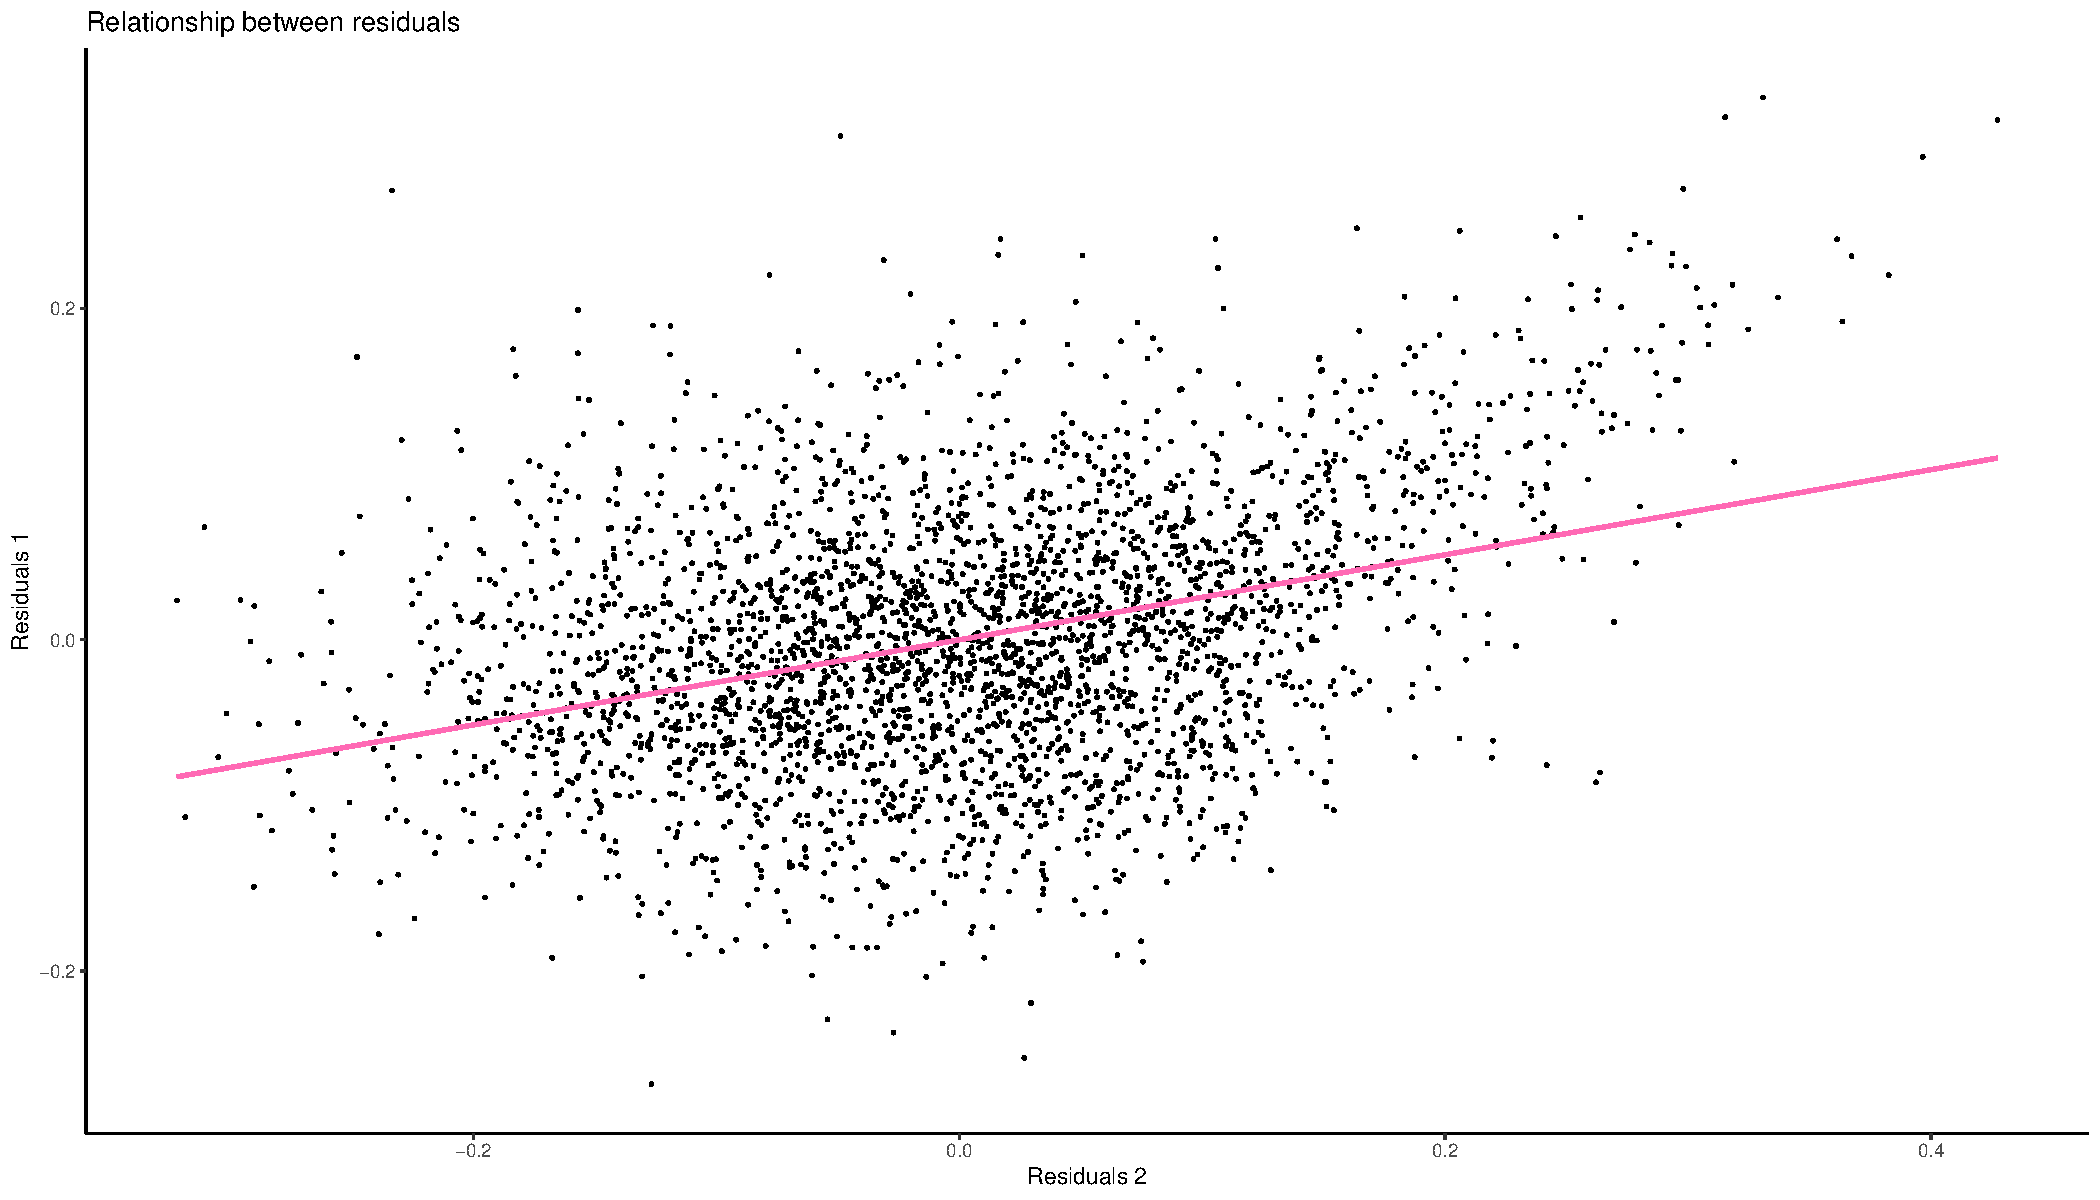
\includegraphics[width=0.95\linewidth]{P3_graph_4.pdf}
			\caption{Relationship between residuals}
		\end{figure}
		
		\item \textbf{Write the prediction equation.}
		
		Using the values of y-intercept and $\hat{\beta}$ estimated from the regression model above, the prediction equation is:
		
		$$\widehat{\text{residuals\_1}} = 0 + 0.26 \cdot \text{residuals\_2}$$
		
	\end{enumerate}
	
	\newpage	

\section*{Question 5}
\noindent \textbf{What if the incumbent's vote share is affected by both the president's popularity and the difference in spending between incumbent and challenger?} 
	\begin{enumerate}
		\item \textbf{Run a regression where the outcome variable is the incumbent's \texttt{voteshare} and the explanatory variables are \texttt{difflog} and \texttt{presvote}.}	\vspace{0cm}
		
		I used the built-in R function \texttt{lm()} to run the regression for Question $5$, using \texttt{voteshare} as the outcome (Y) variable and \texttt{difflog} as the first explanatory (X) variable, and \texttt{presvote} as the second explanatory (X) variable. Here, \texttt{voteshare} is the incumbent's proportion of the vote, whilst \texttt{difflog} is the log difference in campaign spending between the incumbent and the challenger, and \texttt{presvote} is the voteshare of the presidential candidate from the incumbent party.
		
		\lstinputlisting[language=R, firstline=188, lastline=189]{PS03_Solutions_AV.R}  
		
		I estimated that the y-intercept is $0.44864$, $\hat{\beta}_1$ is $0.03554$, and $\hat{\beta}_2$ is $0.25688$. This means that when both \texttt{difflog} and \texttt{presvote} are equal to 0, the predicted \texttt{voteshare} value is $0.45$ (rounded to $2$ d.p.). Furthermore, holding \texttt{presvote} constant, for every one unit increase in \texttt{difflog}, there is a $0.04$ (rounded to $2$ d.p.) expected increase in \texttt{voteshare}; and, holding \texttt{difflog} constant, for every one unit increase in \texttt{presvote}, there is a $0.26$ (rounded to $2$ d.p.) expected increase in \texttt{voteshare}.
		
		\item \textbf{Write the prediction equation.}	\vspace{0cm}
		
		Using the values of y-intercept and $\hat{\beta}_1$ and $\hat{\beta}_2$ estimated above, the prediction equation is:
		
		$$\widehat{\text{voteshare}} = 0.45 + 0.04 \cdot \text{difflog} + 0.26 \cdot \text{presvote}$$ 
		
		\item \textbf{What is it in this output that is identical to the output in Question 4? Why do you think this is the case?}
		
		The $\hat{\beta}$ value in Question $4$ is identical to the $\hat{\beta}_2$ in Question $5$: $0.26$ (rounded to $2$ d.p.). The \texttt{residuals\_1} removes all variation in \texttt{voteshare} explained by \texttt{difflog}. Similarly, the \texttt{residuals\_2} removes all variation in \texttt{presvote} explained by \texttt{difflog}. The regression of these two residuals in Question $4$ thus purely measures the relationship between \texttt{voteshare} and \texttt{presvote}, holding \texttt{difflog} constant.
		
		The multi-variable regression I executed in Question $5$ automatically estimates the $\hat{\beta}$ value for \texttt{presvote} while holding \texttt{difflog} constant. As a result, the $\hat{\beta}$ in Question $4$ is identical to the $\hat{\beta}_2$ in Question $5$.
		
	\end{enumerate}




\end{document}
